\begin{figure}[H]
  \centering
  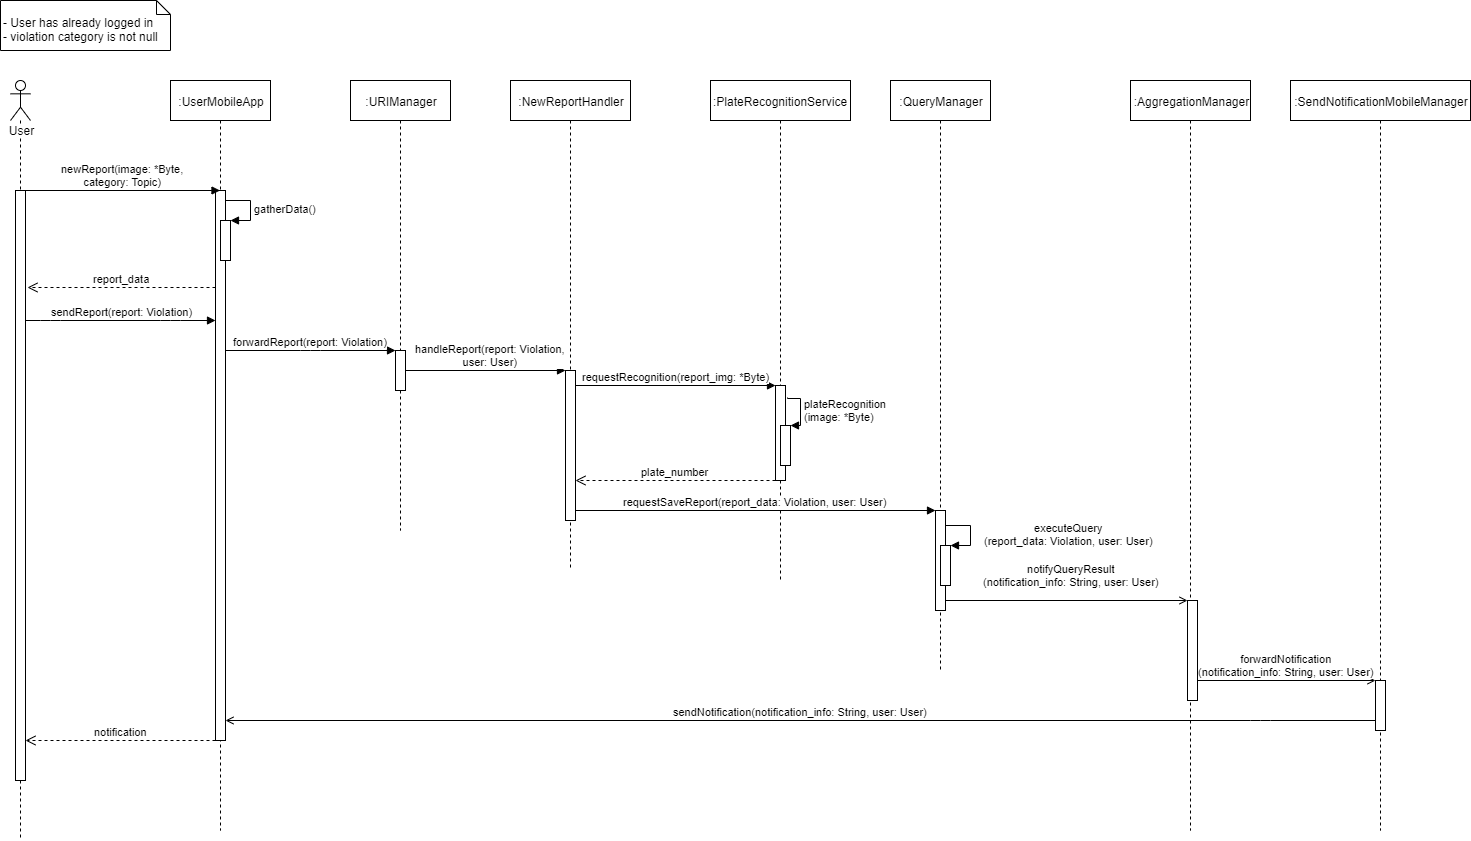
\includegraphics[width=1\textwidth]{Images/UML_diagrams/Sequence_Diagrams/Send_Report_sd.png}
  \caption{Send report sequence diagram}
  \label{fig:send_report_sd}
\end{figure}
This sequence diagram represents the process of the basic functionality of the app, that is to say the send report function. As soon as the user taps on the new report icon, the app opens the camera interface so that the user can take the picture of the violation. Once the picture has been taken the app automatically gather from the phone the required data that need to be associated with the report, such as: GPS coordinates, date and time. Then a page that contains such data and a preview of the picture is shown to the user. In order to send a valid report he must also choose, from a list of violation category, the one that best suits the event; ultimately he can choose to modify the information as he wants (e.g. retake picture, change address, etc ...). Once the report is complete the application submits the report to the URIManager that will forward the request to the NewReportHandler component. This component will send to the PlateRecognitionService component the image in order to retrieve the plate number associated. Once the plate number is returned to the NewReportHandler, the complete report is sent to the QueryManager that will perform an insert query on the database. After the insertion, the latter will send the query result, in this case just a status message (e.g. correct saving), to the AggregationManager that will just forward the notification to the SendMobileNotificationManger. The SendMobileNotificationManger finally sends a push notification to the mobile app containing a message about the correct.
 